\section{Introduction}\label{sec:intro}

\begin{figure*}[t]
\centering
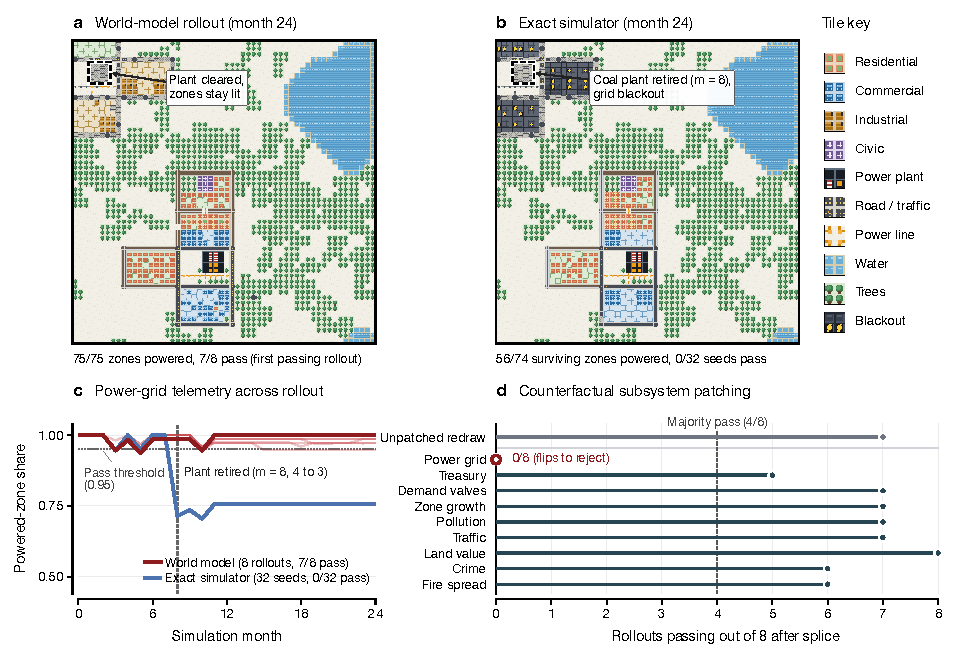
\includegraphics[width=\textwidth]{figures/fig1_environment.pdf}
\caption{\textbf{Demolishing a coal plant causes a simulator blackout while all zones stay powered in the world model.} A \Horizon-month plan executed from the identical initial city in our primary \SizeM{} world model and the exact Micropolis engine. Both demolish a coal plant at month \FigOneDropMonth{}, yet only the true simulator suffers a grid blackout. \textbf{a}, Imagined month-\Horizon{} city for the highest-discrepancy plan among the \RandThouAccRejCount{} exploited plans from \Bp{3} random shooting (Appendix~\ref{app:patching}), rendered with procedural micro-sprites; all zones stay powered and \FigOneEmuPass{} of \FigOneK{} replayed rollouts pass (\FigOneAuditPass{} of \FigOneK{} in the search draw). \textbf{b}, Bit-exact C++ replay in which bulldozing a plant tile retires the plant at month \FigOneDropMonth{}, leaving \FigOneEngOff{} of \FigOneEngZones{} zones unpowered (dark unpowered zones; zero of \OracleSeeds{} oracle seeds pass). \textbf{c}, Powered-zone share across \FigOneK{} imagined rollouts vs.\ \OracleSeeds{} engine seeds following the month-\FigOneDropMonth{} plant demolition (the deterministic capacity cliff yields zero cross-seed spread on the simulator trace). \textbf{d}, Counterfactual subsystem patching (\FigOnePatchK{} rollouts) showing that overwriting the power grid from the engine flips the verdict to zero passes, while all eight other subsystems leave the false pass intact.}
\label{fig:env}
\end{figure*}

\begin{figure*}[t]
\centering
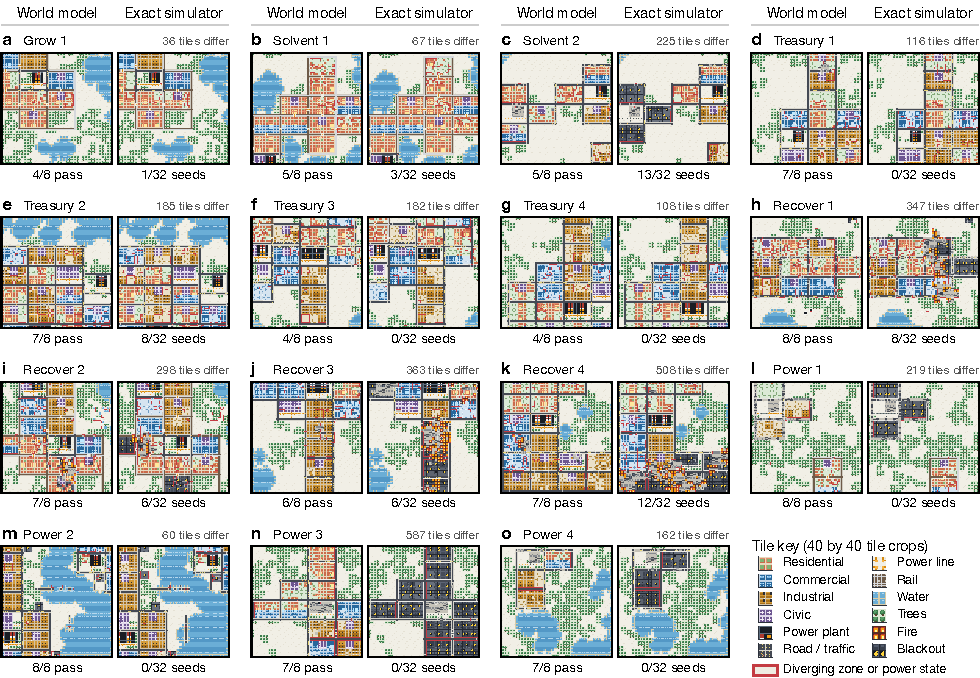
\includegraphics[width=\textwidth]{figures/fig_gallery.pdf}
\caption{\textbf{World-model search selects plans that fail in the exact simulator across all five task families.} \GalPairsWord{} representative plans accepted by the primary world model and rejected by the \OracleSeeds-seed oracle, cropped to the \GalCrop{}-by-\GalCrop{}-tile window of peak structural divergence at month \Horizon{} (\emph{grow} contributes \GalGrowShownWord{} case and \emph{solvent} \GalSolvShownWord{}; Appendix~\ref{app:gallery}). Each pair displays the first passing world-model rollout out of \GalSamples{} draws (left; passing rollouts out of \GalSamples{}) beside the primary exact-simulator replay (right; passing oracle seeds out of \OracleSeeds{}, with white-haloed crimson contours outlining tiles that diverge in structural class or power state), rendered via procedural micro-sprites.}
\label{fig:gallery}
\end{figure*}

Generative world models now serve both as synthetic training arenas for reinforcement learning \citep{hafner2025dreamerv3,alonso2024diamond,hafner2025dreamer4,chen2025dreamgym} and as zero-shot evaluators that rank plans before deployment \citep{quevedo2025worldgym,guo2026ctrlworld,geminirobotics2025veo}. Whenever search or policy gradients select top-scoring imagined trajectories, optimisation concentrates on regions where stochastic luck and systematic model errors align. The broad failure modes are well known. \citet{ha2018worldmodels} showed a controller scoring \HaDream{} inside a learned VizDoom dream collapsing to \HaGame{} in the true game, \citet{lambert2020objective} documented the mismatch between trajectory accuracy and control performance, and recent theory proves imperfect models remain exploitable over rich policy classes \citep{bhamidipaty2026exploitable}. What remains scarce is controlled empirical measurement that benchmarks model-based planning error above finite-sample selection luck, paired with practical pre-training audit evidence \citep{yu2026worldmodelseval}.

Measuring exploitation cleanly requires a baseline that standard evaluations omit. Even inside an exact stochastic simulator, selecting the best plan from finite rollouts introduces upward bias through the \emph{optimiser's curse} \citep{smith2006optimizer}. Separating learned-model degradation from stochastic selection noise requires dynamics rich enough to challenge neural models alongside bit-exact state-and-seed replay. Each optimiser can then run identically inside both the learned model and an \emph{exact-simulator reference} queried on fresh non-oracle seeds.

We build this testbed around Micropolis, the open-source C++ core of the 1989 urban economy simulator\footnote{Micropolis is a registered trademark of Micropolis Corporation (Micropolis GmbH) used under the Micropolis Public Name License \citep{micropolisnamelicense}. We build upon MicropolisCore \citep{micropoliscore} under GPL-3.0 with additional terms \citep{micropolisgpl}, with deterministic replay patches documented in our sources.}. Unlike arcade pixel arenas or smooth rigid-body control, Micropolis couples spatial land-use rules with delayed fiscal accounting and discrete network cutoffs (Figure~\ref{fig:anatomy}). Construction deducts immediately from city reserves. Residential, commercial, and industrial migration follows lagged census valves, and taxes and service budgets settle annually. Depth-first power routing imposes sharp grid cutoffs alongside stochastic disasters. We train a \Ladder-checkpoint ladder of stochastic ConvNeXt U-Net world models across parameter scales, data budgets, and objectives. We then evaluate them from single logged plans and random shooting through \Bp{4}-plan cross-entropy search, monthly replanning, and \RlRunsDone{} PPO runs (Figures~\ref{fig:env} and~\ref{fig:gallery}).

\paragraph{Summary of contributions and findings.}
\begin{itemize}
\item \textbf{Short-horizon fidelity masks task-horizon drift.} Every ladder checkpoint clears one-month changed-tile F1 and \RollA-month scalar gates. Yet at our two-epoch training budget, the primary \SizeM{} model equals or exceeds start-state copying error by month \Horizon{} on \HorRestN{} of \HorOverlays{} spatial overlays (Section~\ref{sec:setting}).
\item \textbf{Search widens ground-truth shortfall beside persistent excess false acceptance.} On the two-epoch ladder, excess false acceptance appears before search and persists across budgets. Scaling adaptive CEM from \Bp{1} to \Bp{4} lifts world-model ground-truth pass rates through \Bp{3} before stalling between \Bp{3} and \Bp{4}, while exact-simulator discovery keeps climbing. This widens the absolute shortfall from \PaTenShort{} to \PaTenThouShort{} (Section~\ref{sec:pressure})\RpFindClause{}. In-imagination PPO shows parallel optimism, while sixfold longer one-step training flips spatial rollouts to zero-acceptance pessimism on \ExtTrZeroAccFams{} of five task families without closing the \Bp{4} shortfall (Section~\ref{sec:extended}).
\item \textbf{Perturbation-controlled patching isolates dynamic blind spots.} Splicing ground-truth subsystems into exploited rollouts shows raw power-grid flips do not exceed conservative random-overwrite controls. By contrast, \FireFindingSentence{} (Section~\ref{sec:where}).
\item \textbf{Single-plan verdict calibration ranks RL exploitation within our model ladder.} Across \AcPairs{} model-task pairs, short-horizon F1, \RollA-month error, and log-likelihood vary narrowly across gate-passing runs and show weak association with exploitation. Scoring one fixed logged plan per starting instance across the \AllCities-city bank instead ranks downstream PPO exploitation at Spearman \AcEOneWithin{} within family and \AcEOneRho{} pooled (Section~\ref{sec:across}).
\item \textbf{Coverage and inference defences distinguish rejecting bad plans from finding good ones.} Single-seed fiscal-coverage retraining cuts pooled CEM excess to \CovAdAllCovExcess{} \ci{\CovAdAllCovExcessCI} without raising ground-truth pass rates or fixing topological power failures (Section~\ref{sec:coverage}). Post-hoc inference defences cut false acceptance only by rejecting \DefSigFalseRejMin{}--\DefSigFalseRejMax{} of truly passing plans under shooting (Section~\ref{sec:defences}).
\end{itemize}
